\begin{figure}[hbt]
	\centering
	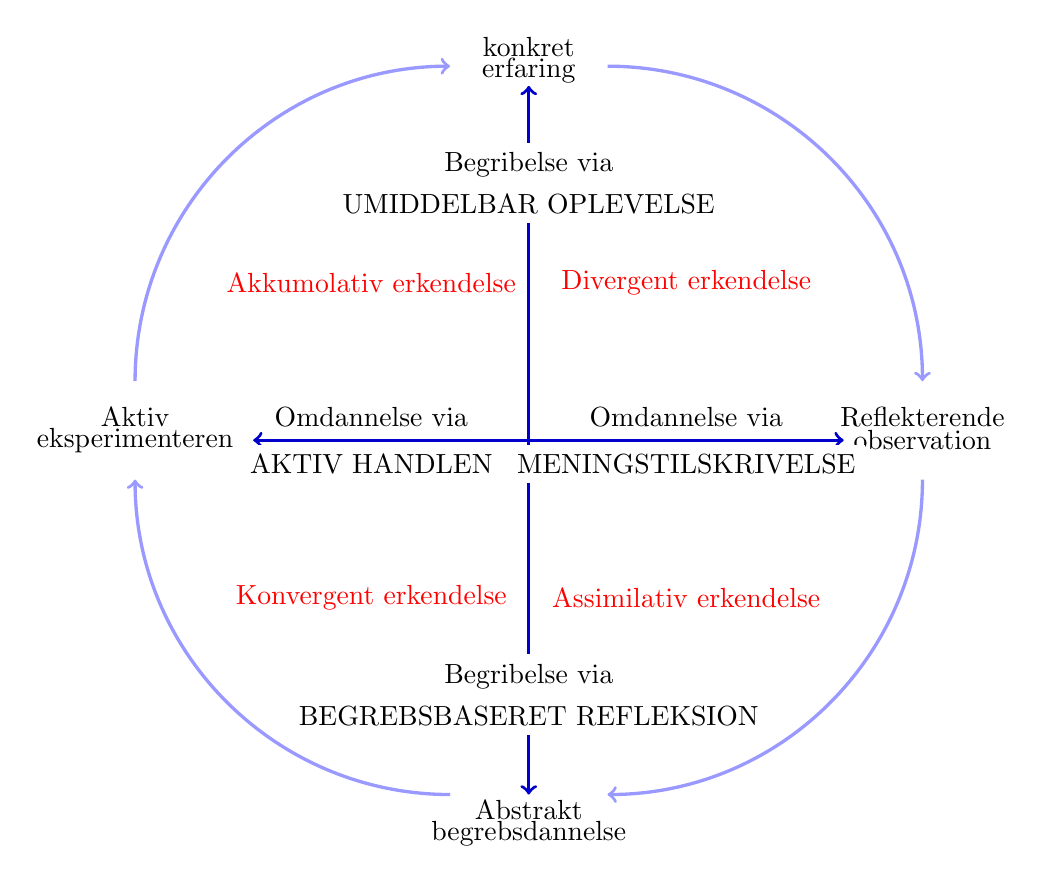
\begin{tikzpicture}
		%\draw[very thin, lightgray, step=1mm] (0,0) grid (10,10);
		%\draw[thin, gray, step=5mm] (0,0) grid (10,10);
		%\draw[thick, darkgray, step=10mm] (0,0) grid (10,10);
		
		% WRITE THE FOUR POINTS
		\node at (0,5.3) {Aktiv};
		\node at (0,5) {eksperimenteren};
		
		\node at (5,10) {konkret};
		\node at (5,9.7) {erfaring};
		
		\node at (10,5.3) {Reflekterende};
		\node at (10,5) {observation};
		
		\node at (5,.3) {Abstrakt};
		\node at (5,0) {begrebsdannelse};
		
		% PLACE ROUND ARROWS
		\draw[very thick, blue!40!white, ->, rotate=-90] (-.5,4) arc (0:-90:4cm);
		\draw[very thick, blue!40!white, ->, rotate=180] (0,-5.75) arc (0:-90:4cm);
		\draw[very thick, blue!40!white, ->, rotate=90] (9.75,-6) arc (0:-90:4cm);
		\draw[very thick, blue!40!white, ->, rotate=0] (10,4.5) arc (0:-90:4cm);

		% DRAW VERTICAL AND HORIZONTAL ARROW
		\draw[very thick, blue!80!black, <->] (5,.5) -- (5,9.5);
		\draw[very thick, blue!80!black, <->] (1.5,5) -- (9,5);
		
		% DRAW NOTES
		\node[draw=white, fill=white, text=black] at (5,2) {Begribelse via};
		\node[draw=white, fill=white, text=black] at (5,1.5) {BEGREBSBASERET REFLEKSION};
		
		\node[draw=white, fill=white, text=black] at (5,8.5) {Begribelse via};
		\node[draw=white, fill=white, text=black] at (5,8.0) {UMIDDELBAR OPLEVELSE};
		
		\node[draw=white, fill=white, text=black] at (3,5.3) {Omdannelse via};
		\node[draw=white, fill=white, text=black] at (3,4.7) {AKTIV HANDLEN};
		
		\node[draw=white, fill=white, text=black] at (7,5.3) {Omdannelse via};
		\node[draw=white, fill=white, text=black] at (7,4.7) {MENINGSTILSKRIVELSE};
		
		\node[red] at (3,7) {Akkumolativ erkendelse};
		\node[red] at (7,7) {Divergent erkendelse};
		\node[red] at (3,3) {Konvergent erkendelse};
		\node[red] at (7,3) {Assimilativ erkendelse};
	\end{tikzpicture}
	\caption[Kolbs l�ringsmodel]{Kolbs l�ringsmodel \citep[side 42]{Kolb:1984} og \citep[side 177]{Gympd}}
	\label{fig:kolb1}
\end{figure}